 \documentclass[journal,12pt,twocolumn]{IEEEtran}
%
\usepackage{setspace}
\usepackage{gensymb}
\singlespacing
\usepackage[cmex10]{amsmath}
\usepackage{amsthm}
\usepackage{mathrsfs}
\usepackage{txfonts}
\usepackage{stfloats}
\usepackage{bm}
\usepackage{cite}
\usepackage{cases}
\usepackage{subfig}
\usepackage{longtable}
\usepackage{multirow}
%\usepackage{algorithm}
\usepackage{enumitem}
\usepackage{mathtools}
\usepackage{steinmetz}
\usepackage{tikz}
\usepackage{circuitikz}
\usepackage{verbatim}
\usepackage{tfrupee}
\usepackage[breaklinks=true]{hyperref}
%\usepackage{stmaryrd}
\usepackage{tkz-euclide} % loads  TikZ and tkz-base
%\usetkzobj{all}
\usetikzlibrary{calc,math}
\usepackage{listings}
    \usepackage{color}                                            %%
    \usepackage{array}                                            %%
    \usepackage{longtable}                                        %%
    \usepackage{calc}                                             %%
    \usepackage{multirow}                                         %%
    \usepackage{hhline}                                           %%
    \usepackage{ifthen}                                           %%
  %optionally (for landscape tables embedded in another document): %%
    \usepackage{lscape}     
\usepackage{multicol}
\usepackage{chngcntr}
%\usepackage{enumerate}

%\usepackage{wasysym}
%\newcounter{MYtempeqncnt}
\DeclareMathOperator*{\Res}{Res}
%\renewcommand{\baselinestretch}{2}
\renewcommand\thesection{\arabic{section}}
\renewcommand\thesubsection{\thesection.\arabic{subsection}}
\renewcommand\thesubsubsection{\thesubsection.\arabic{subsubsection}}
\newcommand\numberthis{\addtocounter{equation}{1}\tag{\theequation}}
\renewcommand\thesectiondis{\arabic{section}}
\renewcommand\thesubsectiondis{\thesectiondis.\arabic{subsection}}
\renewcommand\thesubsubsectiondis{\thesubsectiondis.\arabic{subsubsection}}

% correct bad hyphenation here
\hyphenation{op-tical net-works semi-conduc-tor}
\def\inputGnumericTable{}                                 %%

\lstset{
%language=C,
frame=single, 
breaklines=true,
columns=fullflexible
}


\begin{document}
%


\newtheorem{theorem}{Theorem}[section]
\newtheorem{problem}{Problem}
\newtheorem{proposition}{Proposition}[section]
\newtheorem{lemma}{Lemma}[section]
\newtheorem{corollary}[theorem]{Corollary}
\newtheorem{example}{Example}[section]
\newtheorem{definition}[problem]{Definition}

\newcommand{\BEQA}{\begin{eqnarray}}
\newcommand{\EEQA}{\end{eqnarray}}
\newcommand{\define}{\stackrel{\triangle}{=}}
\bibliographystyle{IEEEtran}
%\bibliographystyle{ieeetr}
\providecommand{\mbf}{\mathbf}
\providecommand{\pr}[1]{\ensuremath{\Pr\left(#1\right)}}
\providecommand{\qfunc}[1]{\ensuremath{Q\left(#1\right)}}
\providecommand{\sbrak}[1]{\ensuremath{{}\left[#1\right]}}
\providecommand{\lsbrak}[1]{\ensuremath{{}\left[#1\right.}}
\providecommand{\rsbrak}[1]{\ensuremath{{}\left.#1\right]}}
\providecommand{\brak}[1]{\ensuremath{\left(#1\right)}}
\providecommand{\lbrak}[1]{\ensuremath{\left(#1\right.}}
\providecommand{\rbrak}[1]{\ensuremath{\left.#1\right)}}
\providecommand{\cbrak}[1]{\ensuremath{\left\{#1\right\}}}
\providecommand{\lcbrak}[1]{\ensuremath{\left\{#1\right.}}
\providecommand{\rcbrak}[1]{\ensuremath{\left.#1\right\}}}
\theoremstyle{remark}
\newtheorem{rem}{Remark}
\newcommand{\sgn}{\mathop{\mathrm{sgn}}}
\providecommand{\abs}[1]{\left\vert#1\right\vert}
\providecommand{\res}[1]{\Res\displaylimits_{#1}} 
\providecommand{\norm}[1]{\left\lVert#1\right\rVert}
%\providecommand{\norm}[1]{\lVert#1\rVert}
\providecommand{\mtx}[1]{\mathbf{#1}}
\providecommand{\mean}[1]{E\left[ #1 \right]}
\providecommand{\fourier}{\overset{\mathcal{F}}{ \rightleftharpoons}}
%\providecommand{\hilbert}{\overset{\mathcal{H}}{ \rightleftharpoons}}
\providecommand{\system}{\overset{\mathcal{H}}{ \longleftrightarrow}}
	%\newcommand{\solution}[2]{\textbf{Solution:}{#1}}
\newcommand{\solution}{\noindent \textbf{Solution: }}
\newcommand{\cosec}{\,\text{cosec}\,}
\providecommand{\dec}[2]{\ensuremath{\overset{#1}{\underset{#2}{\gtrless}}}}
\newcommand{\myvec}[1]{\ensuremath{\begin{pmatrix}#1\end{pmatrix}}}
\newcommand{\mydet}[1]{\ensuremath{\begin{vmatrix}#1\end{vmatrix}}}
\numberwithin{equation}{subsection}
\makeatletter
\@addtoreset{figure}{problem}
\makeatother
\let\StandardTheFigure\thefigure
\let\vec\mathbf
\renewcommand{\thefigure}{\theproblem}
\def\putbox#1#2#3{\makebox[0in][l]{\makebox[#1][l]{}\raisebox{\baselineskip}[0in][0in]{\raisebox{#2}[0in][0in]{#3}}}}
     \def\rightbox#1{\makebox[0in][r]{#1}}
     \def\centbox#1{\makebox[0in]{#1}}
     \def\topbox#1{\raisebox{-\baselineskip}[0in][0in]{#1}}
     \def\midbox#1{\raisebox{-0.5\baselineskip}[0in][0in]{#1}}
\vspace{3cm}
\title{Matrix Theory Assignment 5}
\author{Ritesh Kumar \\ EE20RESCH11005}


\maketitle
\newpage
%\tableofcontents
\bigskip
\renewcommand{\thefigure}{\theenumi}
\renewcommand{\thetable}{\theenumi}
\counterwithout{figure}{section}
\counterwithout{figure}{subsection}
%\begin{document}	
	%	\begin{titlepage}
%	\begin{center}
%		\vspace*{1cm}
%		
%		\textbf{ \huge{Assignment 1}}
%		\vspace{1.5cm}
%		
%		\textbf{Ritesh Kumar} \\
%		textbf{(EE20RESCH11005)}\\
%		\textbf{Communication and Signal Processing}
		\date{Today}
		
%	\end{center}
	%	\end{titlepage}
	\begin{abstract}
		This document demonstrates a method to trace a curve with given equation using matrix algebra.
		\end{abstract}	
	
		Download latex and python codes from 
		\begin{lstlisting}
	https://github.com/Ritesh622/Assignment_EE5609/tree/master/Assignment_5
		\end{lstlisting}	
	\section{Problem Statement} 
	Trace the curve 
	\begin{align}
	\left(x-y\right)^2 = x+y+1
	\label{eq0}
	\end{align}
	
	\section{Solution}	
	
	We have given equation as :
	\begin{align}
\left(x-y\right)^2 = x+y+1
\end{align}	
\begin{align}
\implies x^2  -2xy + y^2 -x - y -1 = 0
\label{eq1}
\end{align}
The general equation of second degree is given by
\begin{align}
ax^2+2bxy+cy^2+2dx+2ey+f=0 \label{eq2}
\end{align}
and can be expressed as
\begin{align}
\vec{x}^T\vec{V}\vec{x}+2\vec{u}^T\vec{x}+f=0 \label{eq3}
\end{align}
where
\begin{align}
\vec{V} &= \vec{V}^T = \myvec{a & b \\ b & c}
\\
\vec{u}^T &= \myvec{d & e}
\end{align}

Comparing \eqref{eq1} with \eqref{eq2}, we get

\begin{align}
\vec{V} &= \vec{V}^T = \myvec{ 1 &  -1 \\ -1 & 1 }
\\
\vec{u}^T &= \myvec{-\frac{1}{2} & - \frac{1}{2}}
\\
f &= -1
\end{align}


Expanding the determinant of V we observe,
\begin{align}
\abs{V} = \mydet{1 & -1 \\ -1 & 1} = 0 \label{eq10}
\end{align}
Also
\begin{align}
\mydet{\vec{V} & \vec{u} \\ \vec{u}^T & f} = 
\mydet{
1 & -1 & -\frac{1}{2} \\ 
-1 & 1 & -\frac{1}{2} \\ 	
-\frac{1}{2} & -\frac{1}{2} & -1}
\neq 0
\label{eq11}
\end{align}

Hence from \eqref{eq10} and \eqref{eq11} we conclude
that given equation is an parabola.The characteristic equation of $\vec{V}$ is given as
follows,


\begin{align}
\mydet{\lambda \vec{I}-\vec{V}} = \mydet{\lambda -1 & -1 \\ -1 & \lambda - 1} &= 0
\\
\implies \left(\lambda - 1 \right)^2 -1 &= 0
\label{eq12}
\end{align}
The eigenvalues are the roots of \eqref{eq12} given by
\begin{align}
\lambda_1 = 0, \lambda_2 = 2
\label{eq13}
\end{align}
The eigenvector $\vec{p}$ is defined as:
\begin{align}
\vec{V} \vec{p}&= \lambda \vec{p}
\\
\implies \brak{\lambda\vec{I}-\vec{V}}\vec{p} &=0
\end{align}
where $\lambda$ is the eigenvalue.  For $\lambda_1$ = 0,
\begin{align}
\vec{V} \vec{p}&=0
\end{align}
Row reducing $\vec{V}$ yields,
\begin{align}
 \myvec{ 1 & -1 \\ -1 & 1} 
\xleftrightarrow{R_2\leftarrow R_2+R_1} 
\myvec{
	1 &  -1 \\ 0 & 0 
} 
\label{eq18}
\end{align}

  Similarly, the eigenvector corresponding to $\lambda_2$ can be obtained as
  
  \begin{align}
  \brak{\lambda_2\vec{I}-\vec{V}}
  = \myvec{ 1 & 1 \\ 1 & 1} 
  \xleftrightarrow{R_2\leftarrow R_2 - R_1} \nonumber   \\
  \myvec{
  	1 & 1   \\ 0 & 0 
  }
  \label{eq19}
  \end{align}
  
  
  

It is easy to verify that 
\begin{align}
\vec{V} &= \vec{P}\vec{D}\vec{P}^{-1}=\vec{P}\vec{D}\vec{P}^T \quad \because \vec{P}^{-1} = \vec{P}^{T} \label{eq:solutions/41/ex1/ellipse_spectrum_eq}
\\
\text{or, } \vec{D} &= \vec{P}^T\vec{V}\vec{P}
\end{align}


From equation \eqref{eq18} and \eqref{eq19}, we have
\begin{align}
\vec{p_1} =  \frac{1}{\sqrt{2}} \myvec{1 \\ 1} 
\text{and},  \vec{p_2} =  \frac{1}{\sqrt{2}} \myvec{1 \\ -1} 
\end{align}
Thus, the eigenvector rotation matrix and the
eigenvalue matrix are 
\begin{align}
\vec{P} &= \frac{1}{\sqrt{2}} \myvec{ \vec{p_1} & \vec{p_2}} = \frac{1}{\sqrt{2}} \myvec{ 1 & 1 \\ 1 & -1} \\
 \vec{D} &= \myvec{0 & 0 \\ 0 & 2} 
\end{align}

\begin{figure}[htb!]	
	\centering	
	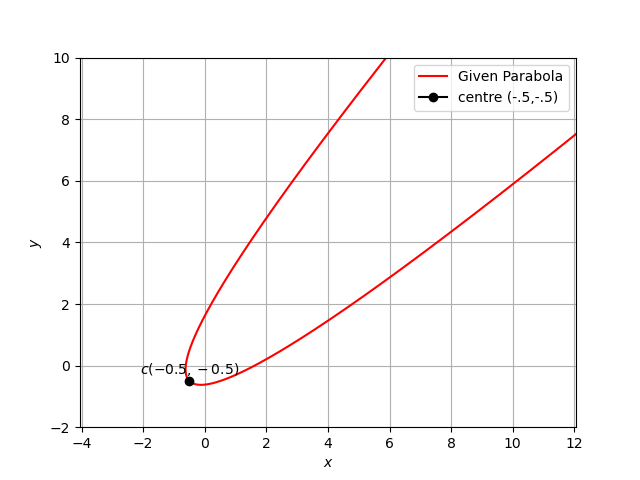
\includegraphics[width=\columnwidth]{parabola.png}	
	\caption{Parabola with the center c}
	\label{fig1}	
\end{figure}

The focal length of the parabola is
given by
\begin{align}
\frac{\mydet{2{\vec{u}}^T\vec{p_1}}}{\lambda_2 } = \frac{\sqrt{2}}{2} = \sqrt{2}
\end{align}
and its equation is
\begin{align}
\vec{y}^T\vec{D}\vec{y} = -2 \eta\myvec{1 & 0 }\vec{y}
\end{align}
where,
\begin{align}
\eta = \vec{u}^T\vec{p_1} = - \frac{1}{\sqrt{2}}
\end{align}

\begin{align}
\myvec{\vec{u}^T + \eta\vec{p_1}^T \\ \vec{V}}c = \myvec{-f \\ \eta\vec{p_1} - \vec{u}} 
\end{align}
\begin{align}
\implies \myvec{ -1 & -1   \\ 1 & -1 \\ -1 & 1 }c = \myvec{1 \\ 0 \\ 0}
\end{align}
Forming the augmented matrix and row reducing
it:


%\begin{align}
%\myvec{-1  &  -1 &  1 \\   1 & -1 &  1 \\  -1 & 1 & 0}  \label{2.30}
%\end{align}

\begin{align}
\myvec{-1  &  -1 &  1 \\   1 & -1 &  1 \\  -1 & 1 & 0}  \label{2.30}
\xleftrightarrow[]{R_2 \leftarrow R_2+R_1  }
%
\myvec{
-1 & -1 & 1 \\ 0 & -2 & 1 \\ -1 & 1 & 0  
} 
\xleftrightarrow[R_1 \leftarrow -1R_1] {R_3 \leftarrow  R_3 - R_1}  \nonumber  \\
%
\myvec{
1 & 1 & -1 \\ 0 & -2 & 1 \\ 0 & 2 & -1 
}
\xleftrightarrow[]{R_3 \leftarrow R_3 +R_2 } 
%	
\myvec{
1 & 1 & -1 \\ 0 & -2 & 1 \\ 0 & 0 & 0 
} \nonumber   \\
\xleftrightarrow[R_1 \leftarrow R_1 -R_2]{R_1 \leftarrow \frac{R_1}{-2}} 
\myvec{
1 & 0 & -\frac{1}{2} \\ 0 & 1 & - \frac{1}{2} \\ 0 & 0 & 0
}
\end{align}
So,
\begin{align}
\vec{c} = \myvec{ -\frac{1}{2} \\ -\frac{1}{2}  } \label{2.31}
\end{align}



\end{document}



